\documentclass[11pt,openany]{book}

% Load packages
\usepackage[utf8]{inputenc} % for unicode input
\usepackage{microtype}
\usepackage{bm}
\usepackage{enumitem}
\usepackage{geometry} % for page layout
\usepackage{hyperref} % for hyperlinks
\usepackage{tocbibind} % includes the bibliography in the table of contents
\usepackage{amsmath, amsfonts, amssymb, amsthm} % for advanced math formatting
\usepackage{lipsum} % generates filler text
\usepackage{fancyhdr}
\usepackage[table]{xcolor} % for cell coloring
\usepackage{graphicx} % for including images
\usepackage{booktabs} % for professional looking tables
\usepackage[normalem]{ulem} % for underlining
\usepackage[document]{ragged2e} % for text alignment
\usepackage{tikz} % for drawing
\usepackage{algorithm}
\usepackage{algpseudocode}
\usepackage{wrapfig}
\usepackage{circuitikz}
\usepackage{caption}
\usepackage{venndiagram}
\usepackage{multicol}
\usepackage{listings}
\usepackage{adjustbox}

% TikZ libraries
\usetikzlibrary{circuits.logic.US, arrows.meta, positioning, calc, fit, decorations.markings, math}

% Document geometry (page size, margins)
\geometry{a4paper, left=20mm, right=20mm, top=25mm, bottom=30mm}

% Custom page style for centered page numbers
\pagestyle{fancy}
\fancyhf{} % Clear all header and footer fields
\fancyhead[RE]{\leftmark} % Left Even pages - Chapter number and name
\fancyhead[RO]{Notes by Ali EL AZDI} % Right Odd pages - Custom message
\fancyfoot[CE,CO]{\thepage} % Centered page number in the footer for both even and odd pages
\renewcommand{\headrulewidth}{0pt}
\renewcommand{\footrulewidth}{0pt}

% Custom commands
\newcommand*\xor{\oplus}
\newcommand{\minidash}{\text{-}}

% Custom spacing command
\makeatletter
\newcommand{\vspacer}[1]{%
  \ifvmode
    \vskip#1\relax
  \else
    \@bsphack
    \vadjust{\vskip#1\relax}
    \@esphack
  \fi
}
\makeatother

%%%%%%%%%%%%%%%%%%% Verilog CODE STYLING %%%%%%%%%%%%%%%%%%%%%%%%%%%%%
\definecolor{keywordcolor}{rgb}{0.5,0.0,0.33}
\definecolor{backgroundcolor}{rgb}{0.95,0.95,1.0}
\definecolor{commentcolor}{rgb}{0.129,0.384,0.529}
\definecolor{stringcolor}{rgb}{0.16,0.00,1.00}
\definecolor{rulecolor}{rgb}{0.46,0.43,0.5}
\definecolor{codegray}{rgb}{0.5,0.5,0.5}

\lstdefinestyle{verilogstyle}{
  language=Verilog,
  basicstyle=\ttfamily\footnotesize,
  backgroundcolor=\color{backgroundcolor},
  commentstyle=\color{commentcolor}\ttfamily, % Add \ttfamily to ensure comments are in typewriter font
  morecomment=[l][\color{commentcolor}\ttfamily]{//}, % Line comment in Verilog
  morecomment=[s][\color{commentcolor}\ttfamily]{/*}{*/}, % Block comments in Verilog
  morekeywords={module, input, output, wire, endmodule, endcase, default, tri, assign, always, if, else, begin, end, case, endcase, parameter}, % Add Verilog keywords
  keywordstyle=\color{keywordcolor},
  stringstyle=\color{stringcolor},
  showstringspaces=false,
  frame=single,
  rulecolor=\color{rulecolor}, % Frame color
  breaklines=true,
  numbers=left,
  numberstyle=\tiny\color{codegray},
  tabsize=2
}

\lstnewenvironment{verilog}
  {\lstset{style=verilogstyle}}
  {}

%%%%%%%%%%%%%%%%%%% C CODE STYLING %%%%%%%%%%%%%%%%%%%%%%%%%%%%%
\definecolor{ckeywordcolor}{rgb}{0.8,0.1,0.1}
\definecolor{cbackgroundcolor}{rgb}{0.95,0.95,0.95}
\definecolor{ccommentcolor}{rgb}{0.0,0.5,0.0}
\definecolor{cstringcolor}{rgb}{0.1,0.1,0.8}
\definecolor{crulecolor}{rgb}{0.5,0.5,0.5}
\definecolor{ccodegray}{rgb}{0.6,0.6,0.6}

\lstdefinestyle{cstyle}{
  language=C,
  basicstyle=\ttfamily\footnotesize,
  backgroundcolor=\color{cbackgroundcolor},
  commentstyle=\color{ccommentcolor}\ttfamily,
  keywordstyle=\color{ckeywordcolor},
  stringstyle=\color{cstringcolor},
  showstringspaces=false,
  frame=single,
  rulecolor=\color{crulecolor},
  breaklines=true,
  numbers=left,
  numberstyle=\tiny\color{ccodegray},
  tabsize=2
}

\lstnewenvironment{cc}
  {\lstset{style=cstyle}}
  {}

%%%%%%%%%%%%%%%%%%% Assembly CODE STYLING %%%%%%%%%%%%%%%%%%%%%%%%%%%%%
\definecolor{akeywordcolor}{rgb}{0.0, 0.2, 0.4}
\definecolor{abackgroundcolor}{rgb}{0.98, 0.99, 1.0}
\definecolor{acommentcolor}{rgb}{0.0, 0.4, 0.6}
\definecolor{astringcolor}{rgb}{0.2, 0.4, 0.8}
\definecolor{arulecolor}{rgb}{0.6, 0.7, 0.8}
\definecolor{acodegray}{rgb}{0.3, 0.4, 0.5}

\lstdefinestyle{assembly}{
  language=[x86masm]Assembler,
  basicstyle=\ttfamily\footnotesize,
  backgroundcolor=\color{abackgroundcolor},
  commentstyle=\color{acommentcolor}\ttfamily,
  keywordstyle=\color{akeywordcolor},
  stringstyle=\color{astringcolor},
  showstringspaces=false,
  frame=single,
  rulecolor=\color{arulecolor},
  breaklines=true,
  numbers=left,
  numberstyle=\tiny\color{acodegray},
  tabsize=2,
  morekeywords={li, and, add, addi, srli, bne}
}

\lstnewenvironment{assembly}
  {\lstset{style=assembly}}
  {}

%%%%%%%%%%%%%%%%%%%%%%%%%%%%%%%%%%%%%%%%%%%%%%%%%%%%%%%%
% Document begins
\begin{document}



% Title Page
\begin{titlepage}
    \centering
    \vspace*{1cm}
    \Huge
    Computer Architecture \newline
    \vspace{10px}
    \LARGE IN BA3 - Paolo IENNE
    \vspace*{10px}
    \newline
    \Large Notes by Ali EL AZDI

    \vfill
    \large
    September 11, 2024
\end{titlepage}

\begin{center}
    \vspace*{1cm}
    \textbf{Introduction}
    \newline
    \paragraph[short]{}{This document is designed to offer a LaTeX-styled overview of the Computer Architecture course, emphasizing brevity and clarity. Should there be any inaccuracies or areas for improvement, please reach out at ali.elazdi@epfl.ch for corrections. For the latest version, check my GitHub repository.}
    \newline
   \url{
        https://github.com/elazdi-al/comparch/blob/main/main.pdf
    }
    \newline
\end{center}

% Table of Contents
\tableofcontents

 % Including chapter0.tex from chapters folder
\chapter{Part I(a) - ISA Reminder, Assembly Language, Compiler - W 1.1}
\textbf{hum...welcome back} \newline
\textit{In the first part of the course, professor introduced (for motivational purposes) how computer architecture, specifically processors, have become essential to our lives, and how the field is growing exponentially. (didn't think it was essential to mention here...)}

\section{From High Level Languages to Assembly Language}
\subsection{High Level Languages}
\textit{When talking about programming we usually think of programs that look like this\dots} \newline \vspace*{5px}

\begin{minipage}[htp]{0.4\textwidth} % Use \textwidth to ensure it spans the page width
\begin{cc}
int data = 0x00123456;
int result = 0;
int mask = 1;
int count = 0;
int temp = 0;
int limit = 32;
do {
    temp = data & mask;
    result = result + temp;
    data = data >> 1;
    count = count + 1;
} while (count != limit);
\end{cc}
\end{minipage}
\hfill
\vline
\hfill
\begin{minipage}[htp]{0.4\textwidth}
    \centering
    \begin{tabular}{|c|c|}
        \hline
        \textbf{name} & \textbf{value} \\ \hline
        data       & 0x00123456  \\ \hline
        result     & 0           \\ \hline
        mask       & 1           \\ \hline
        count      & \dots       \\ \hline
        temp       &             \\ \hline
        limit      &             \\ \hline
        \dots      &             \\ \hline
        my\_float  & 3.141529    \\ \hline
        a\_string  & Hello world! \\ \hline
        \end{tabular}
\end{minipage}

\subsection{Assembly Language}
We use this code because it enables us to build a \textit{Finite State Machine}, which isn't feasible with C code. This language provides a more rigid format with a sequence of numbered instructions, an \textit{opcode}, predefined variable names, and the ability to \textbf{jump between lines}.
\newpage
\begin{center}
    \begin{assembly}
    li x1, 0x00123456
    li x2, 0
    li x3, 1
    li x4, 0
    li x5, 0
    li x6, 32
loop: and x5, x1, x3
    add x2, x2, x5
    srli x1, x1, 1
    addi x4, x4, 1
    bne x4, x6, loop
    \end{assembly}
\end{center}

\section{Processors}
\textbf{Remember, a processor can be decomposed into five components:} \newline
\begin{itemize}[noitemsep]
    \item[-] \textbf{ALU (Arithmetic and Logic Unit)}: Performs arithmetic and logical operations.
    \item[-] \textbf{Register File}: Stores data temporarily for quick access during processing.
    \item[-] \textbf{Memory}: Holds data and instructions needed by the processor.
    \item[-] \textbf{Control Logic}: Directs the operation of the processor by coordinating the other components.
    \item[-] \textbf{PC (Program Counter)}: Keeps track of the address of the next instruction to be executed.
    \item[-] \textbf{Instruction Memory}: Stores the program instructions that the processor will execute.
\end{itemize}
\begin{center}
    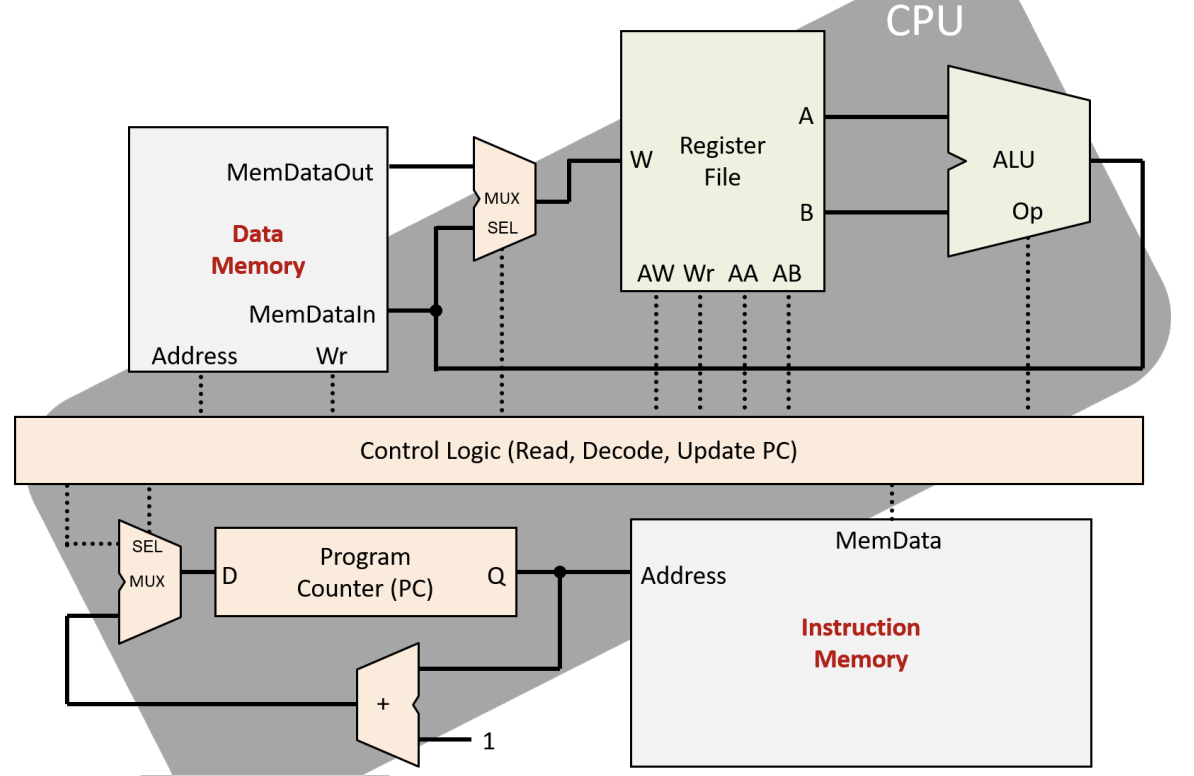
\includegraphics[width=0.5\textwidth]{chapters/chapter1/images/processor.png}
\end{center}

We may distinguish three types of general operations made by the processor: \newline
\subsubsection*{Encoding}
\begin{center}
    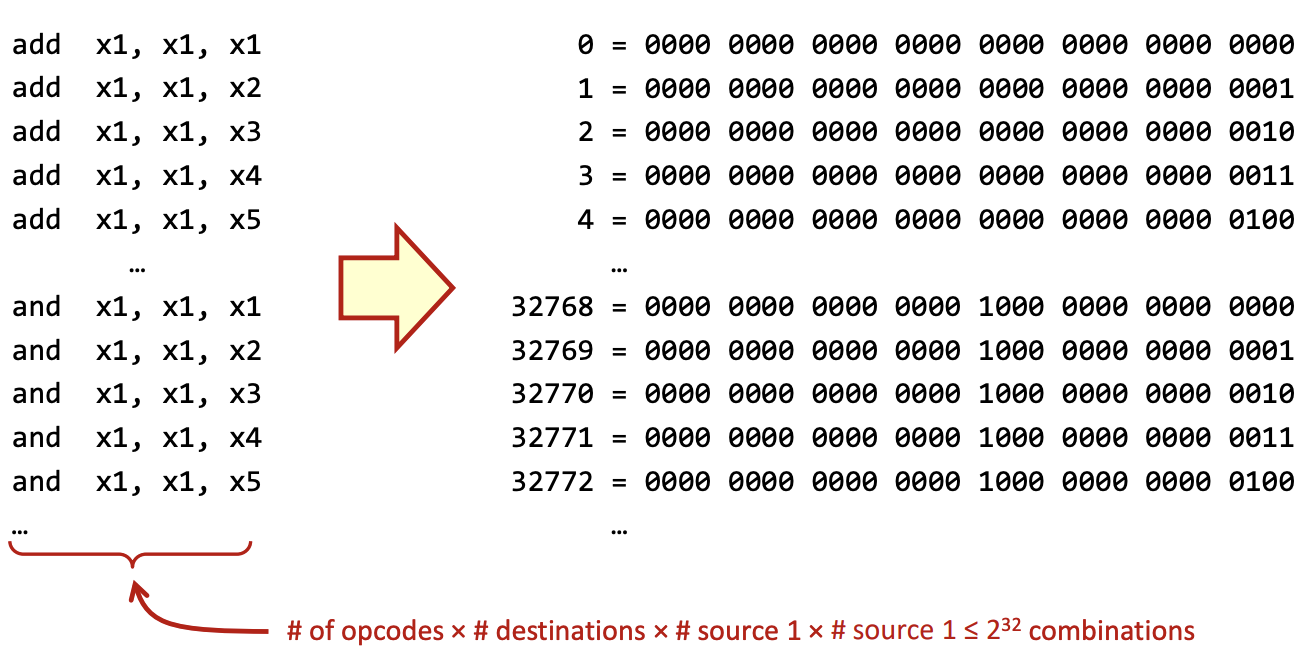
\includegraphics[width=0.65\textwidth]{chapters/chapter1/images/encoding.png}
\end{center}
\subsubsection*{Fetching}
\begin{center}
    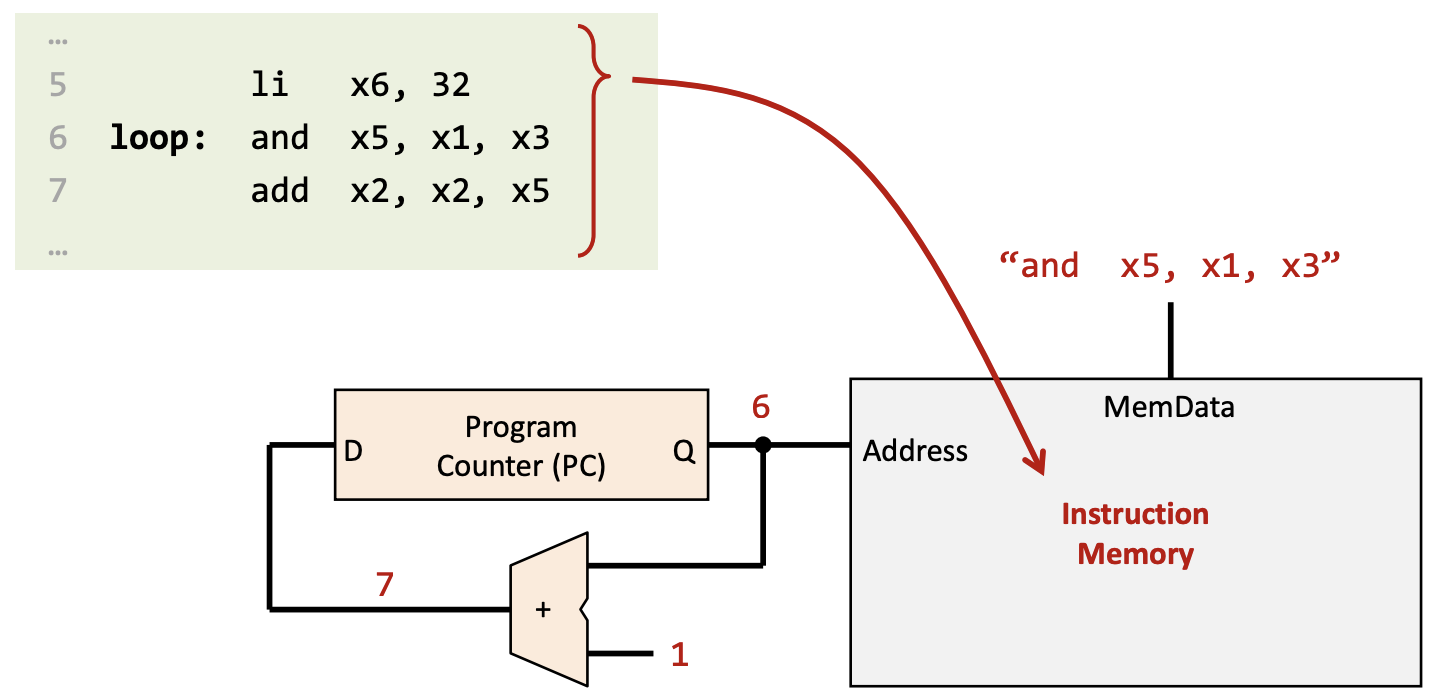
\includegraphics[width=0.65\textwidth]{chapters/chapter1/images/fetching.png}
\end{center}
\subsubsection*{Executing}
\begin{center}
    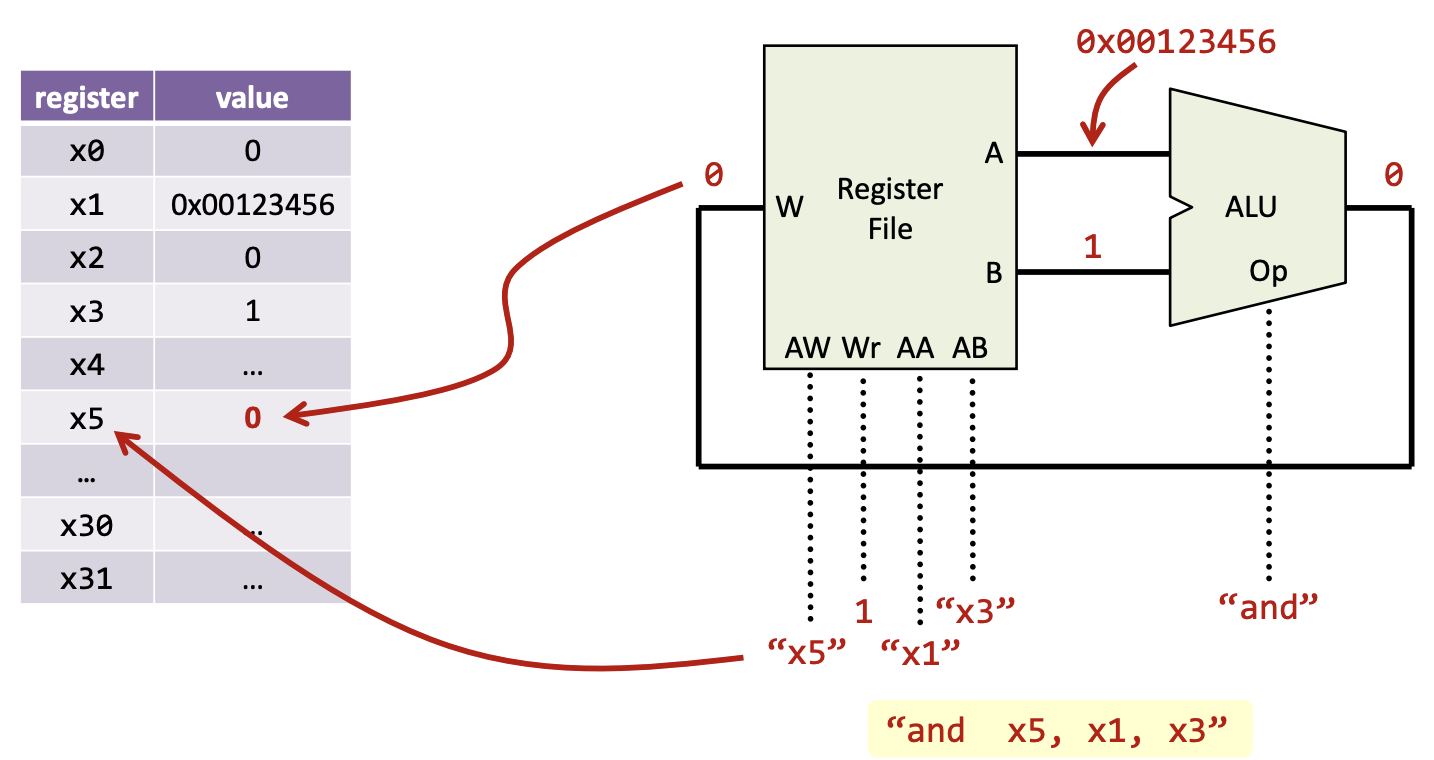
\includegraphics[width=0.65\textwidth]{chapters/chapter1/images/executing.png}
\end{center}


\section{Joint or Disjoint Program and Data Memories}
\textit{There are two main types of architectures one called the Harvard Architecture (Where the data and the memory are seperate) and pne called Unified Architecture (where data is shared with the program memory)} \newline
\vspace*{5px}
\begin{minipage}[htp]{0.4\textwidth}
    \texttt{Harvard Architecture} \newline
    \vspace*{2px}
    \centering
    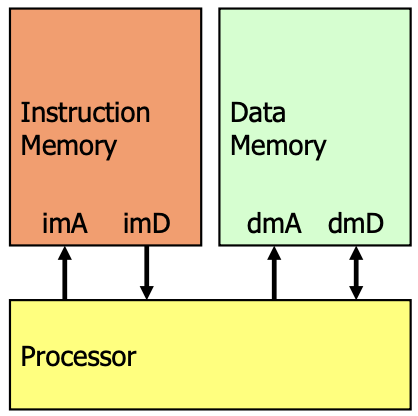
\includegraphics[width=0.6\textwidth]{chapters/chapter1/images/harvard.png}
\end{minipage}
\hfill
\vline
\hfill
\begin{minipage}[htp]{0.4\textwidth}
    \texttt{Unified Architecture} \newline    
    \vspace*{2px}

    \centering
    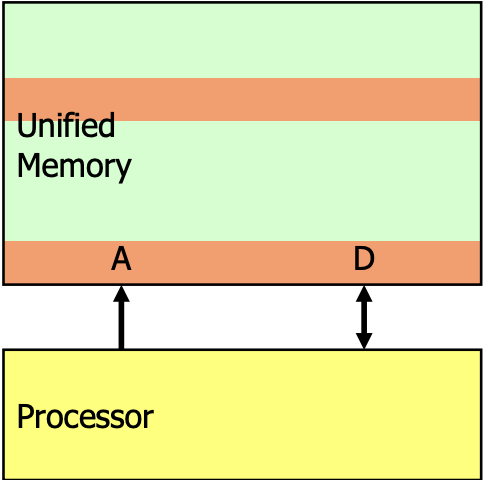
\includegraphics[width=0.6\textwidth]{chapters/chapter1/images/unified.png}
\end{minipage}
\newpage
\section{The Encoding problem}
\textit{We may ask ourselves how we encode assembly written instructions into actual 0s and 1s.} \newline
\subsection{The Stupid Solution}
\textit{Now, the professor throws out the "stupid idea"(his words) of just counting all possible instructions, assigning a number to each one, and writing the numbers in binary. The problem with such a method is that the number of instructions could grow exponentially, requiring an unmanageable number of bits to represent each one, leading to inefficiency.} \newline 
\begin{center}
    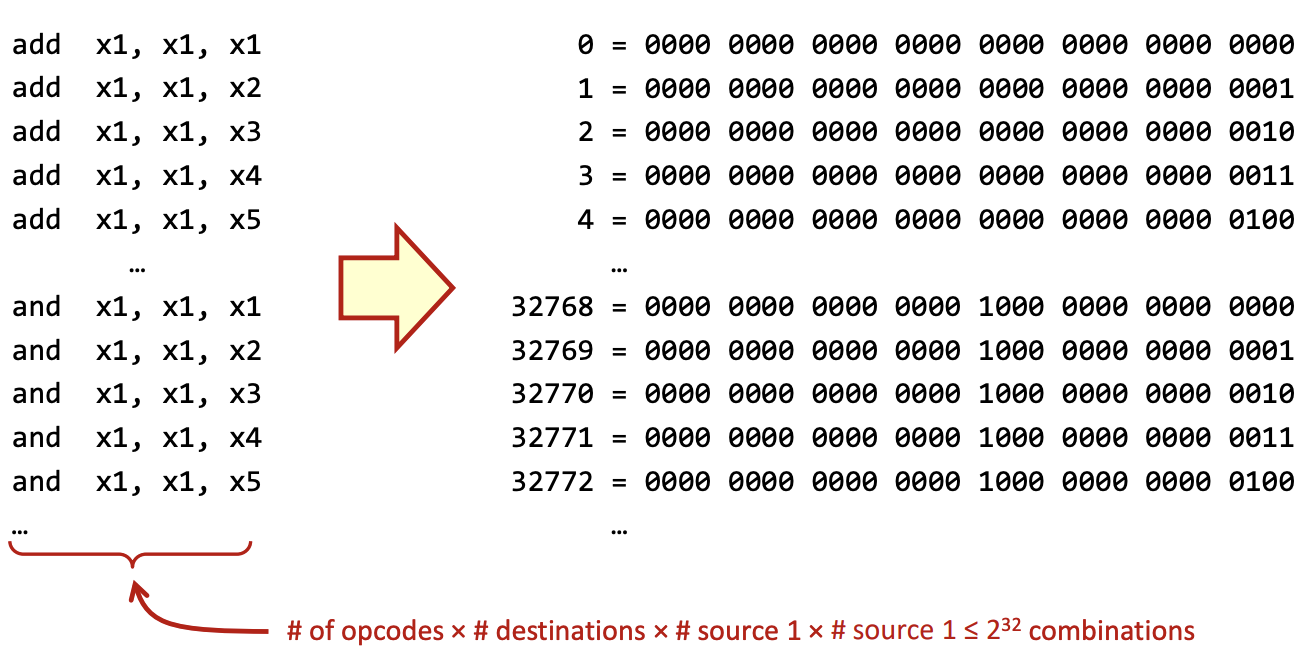
\includegraphics[width=0.7\textwidth]{chapters/chapter1/images/encoding.png}
    \centering
    \textbf{"stupid solution"}
\end{center}

\subsection{RISC-V Encoding (The Solution)}
\textbf{Instead, the chosen solution is to use an instruction set encoding where instructions are grouped into classes, each with a fixed format. This approach optimizes both memory usage and processing speed by limiting the number of bits required to represent instructions, while still allowing for a large variety of operations.} \newline
\begin{center}
    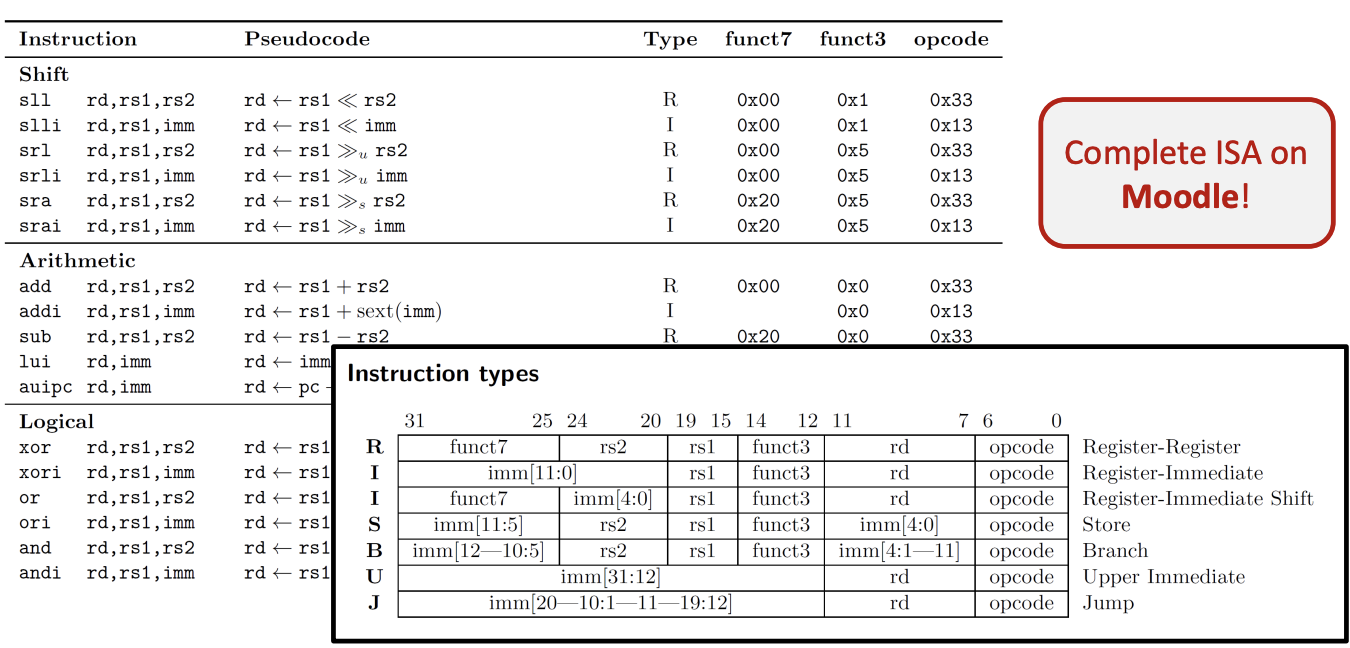
\includegraphics[width=0.7\textwidth]{chapters/chapter1/images/riscv.png}
    \centering
    \textbf{RISC-V encoding}
\end{center}

\newpage
\subsection{Automating this process}
\subsubsection{Assembler}
\textit{The program that does this is called an assembler. It takes the assembly code and converts it into machine code.} \newline
\begin{center}
    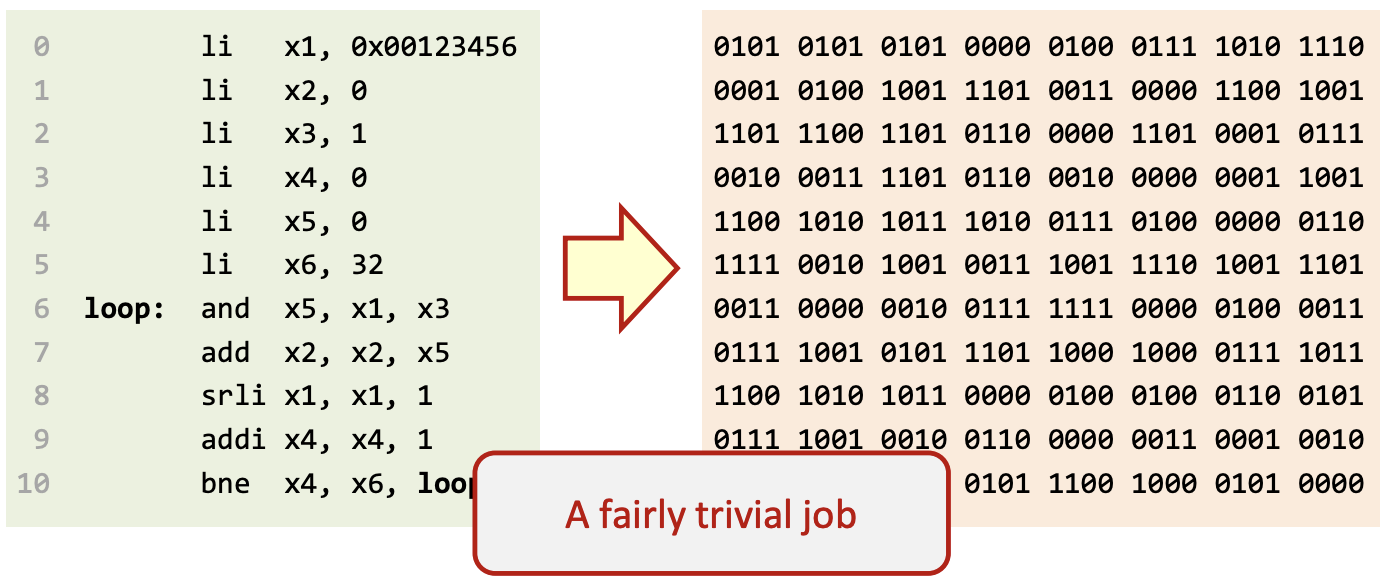
\includegraphics[width=0.7\textwidth]{chapters/chapter1/images/assembler.png}
    \centering
    \textbf{Assembly}
\end{center}
\subsubsection{Compiler}
A compiler is a program that translates high-level source code written in languages like C or Java into machine code or an intermediate representation. This machine code can then be executed by the processor. The compiler performs various stages, such as lexical analysis, parsing, optimization, and code generation, ensuring that the program runs efficiently on the target hardware.
\begin{center}
    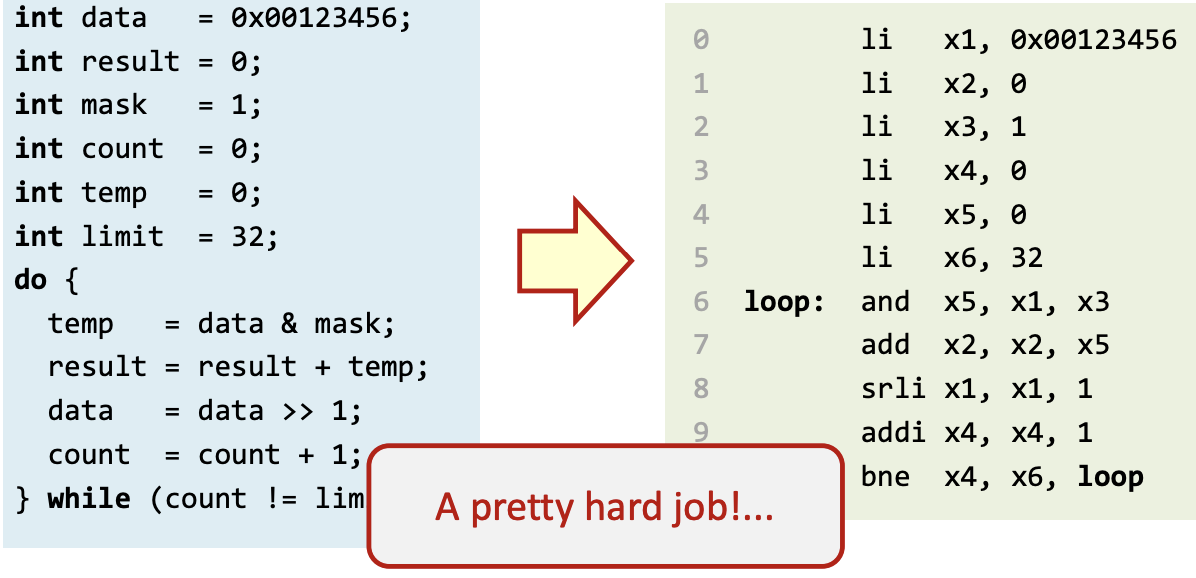
\includegraphics[width=0.7\textwidth]{chapters/chapter1/images/compiler.png}
    \centering
    \textbf{Compilation}
\end{center}

\newpage
\section{ISA (Instruction Set Architecture)}
\textit{The ISA is the interface between the hardware and the software. It defines the instructions that a processor can execute, as well as the format of those instructions.} \newline
\begin{center}
    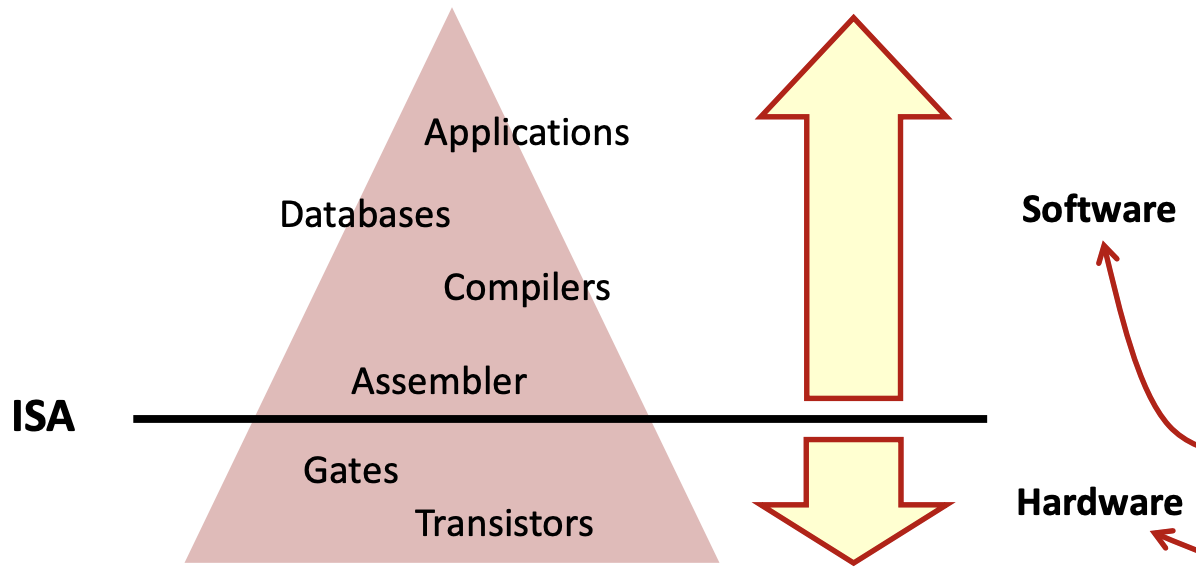
\includegraphics[width=0.65\textwidth]{chapters/chapter1/images/isa.png}
    \centering
\end{center} % Including chapter0.tex from chapters folder



\end{document}
